\documentclass[a4paper,12pt]{article}
\usepackage{tikz}
\usetikzlibrary{arrows}
\usetikzlibrary{automata}
\usetikzlibrary{backgrounds}
\usetikzlibrary{decorations}
\begin{document}
\pagestyle{empty}
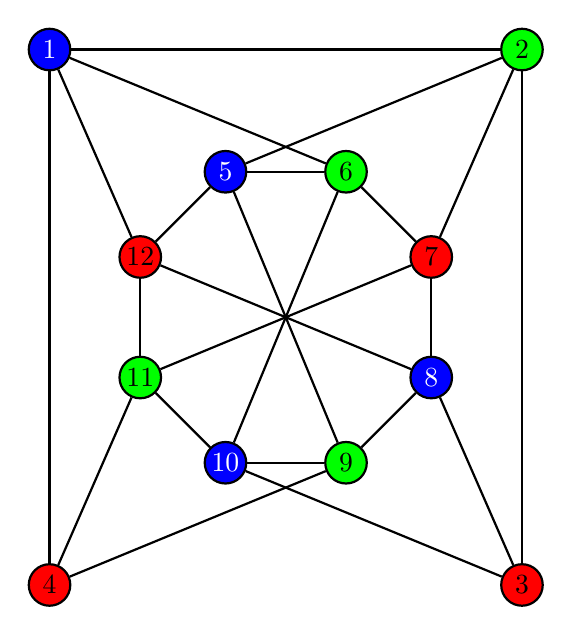
\begin{tikzpicture}[scale=2.0]
    \tikzstyle{edge}=[draw=black,thick,-]
    \tikzstyle{node}=[circle,thick,draw=black,fill=white,minimum size=15pt,inner sep=0pt]

    \tikzstyle{red}=[text=black,fill=red]
    \tikzstyle{green}=[text=black,fill=green]
    \tikzstyle{blue}=[text=white,fill=blue]

    \def\x{0.382683}
    \def\y{0.923879}

    \def\X{1.5}
    \def\Y{1.7}

    \node[node,blue]  (x1)  at (-\X, \Y) {$1$};
    \node[node,green] (x2)  at ( \X, \Y) {$2$};
    \node[node,red]   (x3)  at ( \X,-\Y) {$3$};
    \node[node,red]   (x4)  at (-\X,-\Y) {$4$};
    \node[node,blue]  (x5)  at (-\x, \y) {$5$};
    \node[node,green] (x6)  at ( \x, \y) {$6$};
    \node[node,red]   (x7)  at ( \y, \x) {$7$};
    \node[node,blue]  (x8)  at ( \y,-\x) {$8$};
    \node[node,green] (x9)  at ( \x,-\y) {$9$};
    \node[node,blue]  (x10) at (-\x,-\y) {$10$};
    \node[node,green] (x11) at (-\y,-\x) {$11$};
    \node[node,red]   (x12) at (-\y, \x) {$12$};

    \path[edge] (x1) -- (x2);
    \path[edge] (x1) -- (x4);
    \path[edge] (x1) -- (x6);
    \path[edge] (x1) -- (x12);

    \path[edge] (x2) -- (x3);
    \path[edge] (x2) -- (x5);
    \path[edge] (x2) -- (x7);

    \path[edge] (x3) -- (x8);
    \path[edge] (x3) -- (x10);

    \path[edge] (x4) -- (x9);
    \path[edge] (x4) -- (x11);

    \path[edge] (x5) -- (x6);
    \path[edge] (x6) -- (x7);
    \path[edge] (x7) -- (x8);
    \path[edge] (x8) -- (x9);
    \path[edge] (x9) -- (x10);
    \path[edge] (x10) -- (x11);
    \path[edge] (x11) -- (x12);
    \path[edge] (x12) -- (x5);

    \path[edge] (x5) -- (x9);
    \path[edge] (x6) -- (x10);
    \path[edge] (x7) -- (x11);
    \path[edge] (x8) -- (x12);
\end{tikzpicture}
\end{document}

